\subfloat[Baseline\_TF]{
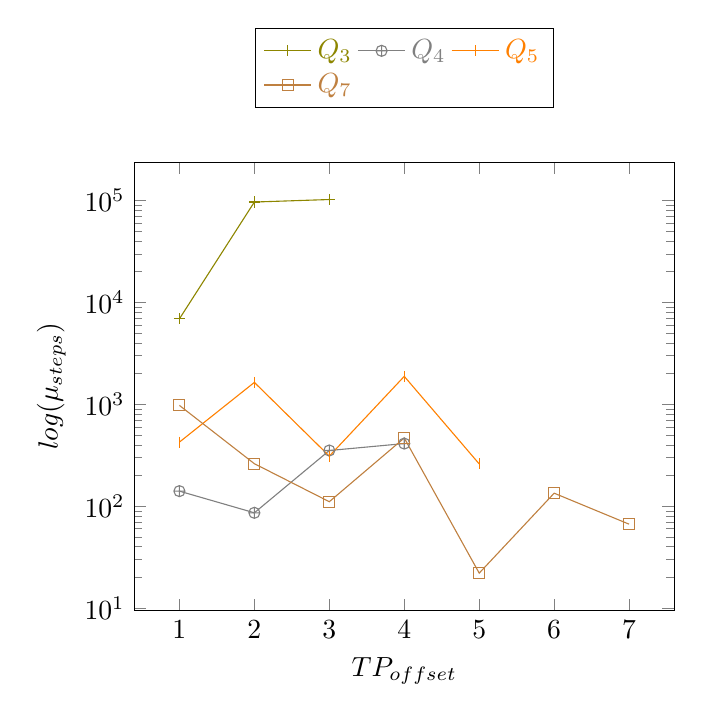
\begin{tikzpicture}\begin{semilogyaxis}[xlabel=$TP_{offset}$,
ylabel=$log(\mu_{steps})$,
  legend entries={
% [blue]$Q_2$,
   [olive]$Q_3$,
   [gray]$Q_4$,
   [orange]$Q_5$,
% [purple]$Q_6$,
   [brown]$Q_7$,
%   [pink]$Q_8$,
%   [yellow]$Q_9$,
 [black]$Q_{11}$,
% [green]$Q_{13}$,
  },
  legend columns=3,
legend style={at={(0.5,1.3)},anchor=north}]
\addplot[mark=+, style=solid, color=olive] coordinates
{ (1, 6895.0714285714275) (2, 96647.14285714287) (3, 102278.28571428571) };
\addplot[mark=oplus, style=solid, color=gray] coordinates
{ (1, 140.33333333333334) (2, 86.0) (3, 351.6666666666667) (4, 411.3333333333333) };
\addplot[mark=|, style=solid, color=orange] coordinates
{ (1, 425.0) (2, 1639.3333333333335) (3, 309.66666666666663) (4, 1879.3333333333335) (5, 259.66666666666663) };
\addplot[mark=square, style=solid, color=brown] coordinates
{ (1, 975.0) (2, 261.0) (3, 110.5) (4, 466.5) (5, 22.0) (6, 134.0) (7, 66.5) };
%\addplot[mark=asterix, style=solid, color=black] coordinates
%{ (1, 0.0) (2, 39.0) (3, 2.0) (4, 0.0) (5, 39.0) (6, 413.0) (7, 2.0) (8, 0.0) (9, 7299.0) (10, 2.0) (11, 39.0) };
\end{semilogyaxis}\end{tikzpicture}
}
